%Se deben explicar todas las pruebas de sintonización manual realizadas. Para esto debe usar la estructura que se adjunta abajo.\\

Para la presente sección, se requiere de una configuración inicial,
para poder comenzar a evaluar el rendimiento del algoritmo para
cada situación donde se quiera sintonizar manualmente algún parámetro.

Los valores de la configuración inicial están dado en base a la experiencia
del trabajo pasado, es decir, en la \emph{primera implementación}.

\begin{itemize}
	\item \texttt{POP = 20}
	\item \texttt{GENS = 200}
	\item \texttt{clonationFactor = 0.4}
	\item \texttt{clonationRate = 0.5}
	\item \texttt{replaceRate = 0.6}
\end{itemize}

Complementariamente, se han considerado tres instancias provenientes de la CSPlib~\cite{CSP}
más precisamente de la sección \emph{``30 new hard problems from Caroline Gagne ''},
donde se han escogido tomando en cuenta el mejor resultado encontrado.
Las instancias son:

\begin{center}
	\begin{tabular}{|l|c|}
	\hline
	\textbf{Instancia} & \textbf{Mejor resultado conocido} \\\hline
	\texttt{pb\_200\_01.txt} & 0 \\\hline
	\texttt{pb\_200\_09.txt} & 10 \\\hline
	\texttt{pb\_200\_10.txt} & 19 \\\hline
	\end{tabular}
\end{center}
\newpage
\subsubsection{Tamaño de población}

\textbf{Prueba}: \blue{prueba1}\\

\textbf{Parámetros involucrados:} Tamaño de población \texttt{(POP)}.\\

\textbf{Objetivo:} Analizar el comportamiento de acuerdo a fitness y tiempo de ejecución del parámetro en un rango de valores.\\

\textbf{Metodología:} Se probarán varios valores en el rango de valores del parámetro \blue{[10,210]}.\\

\textbf{Gráfico:}\\

\begin{figure}[h!]
\begin{center}
	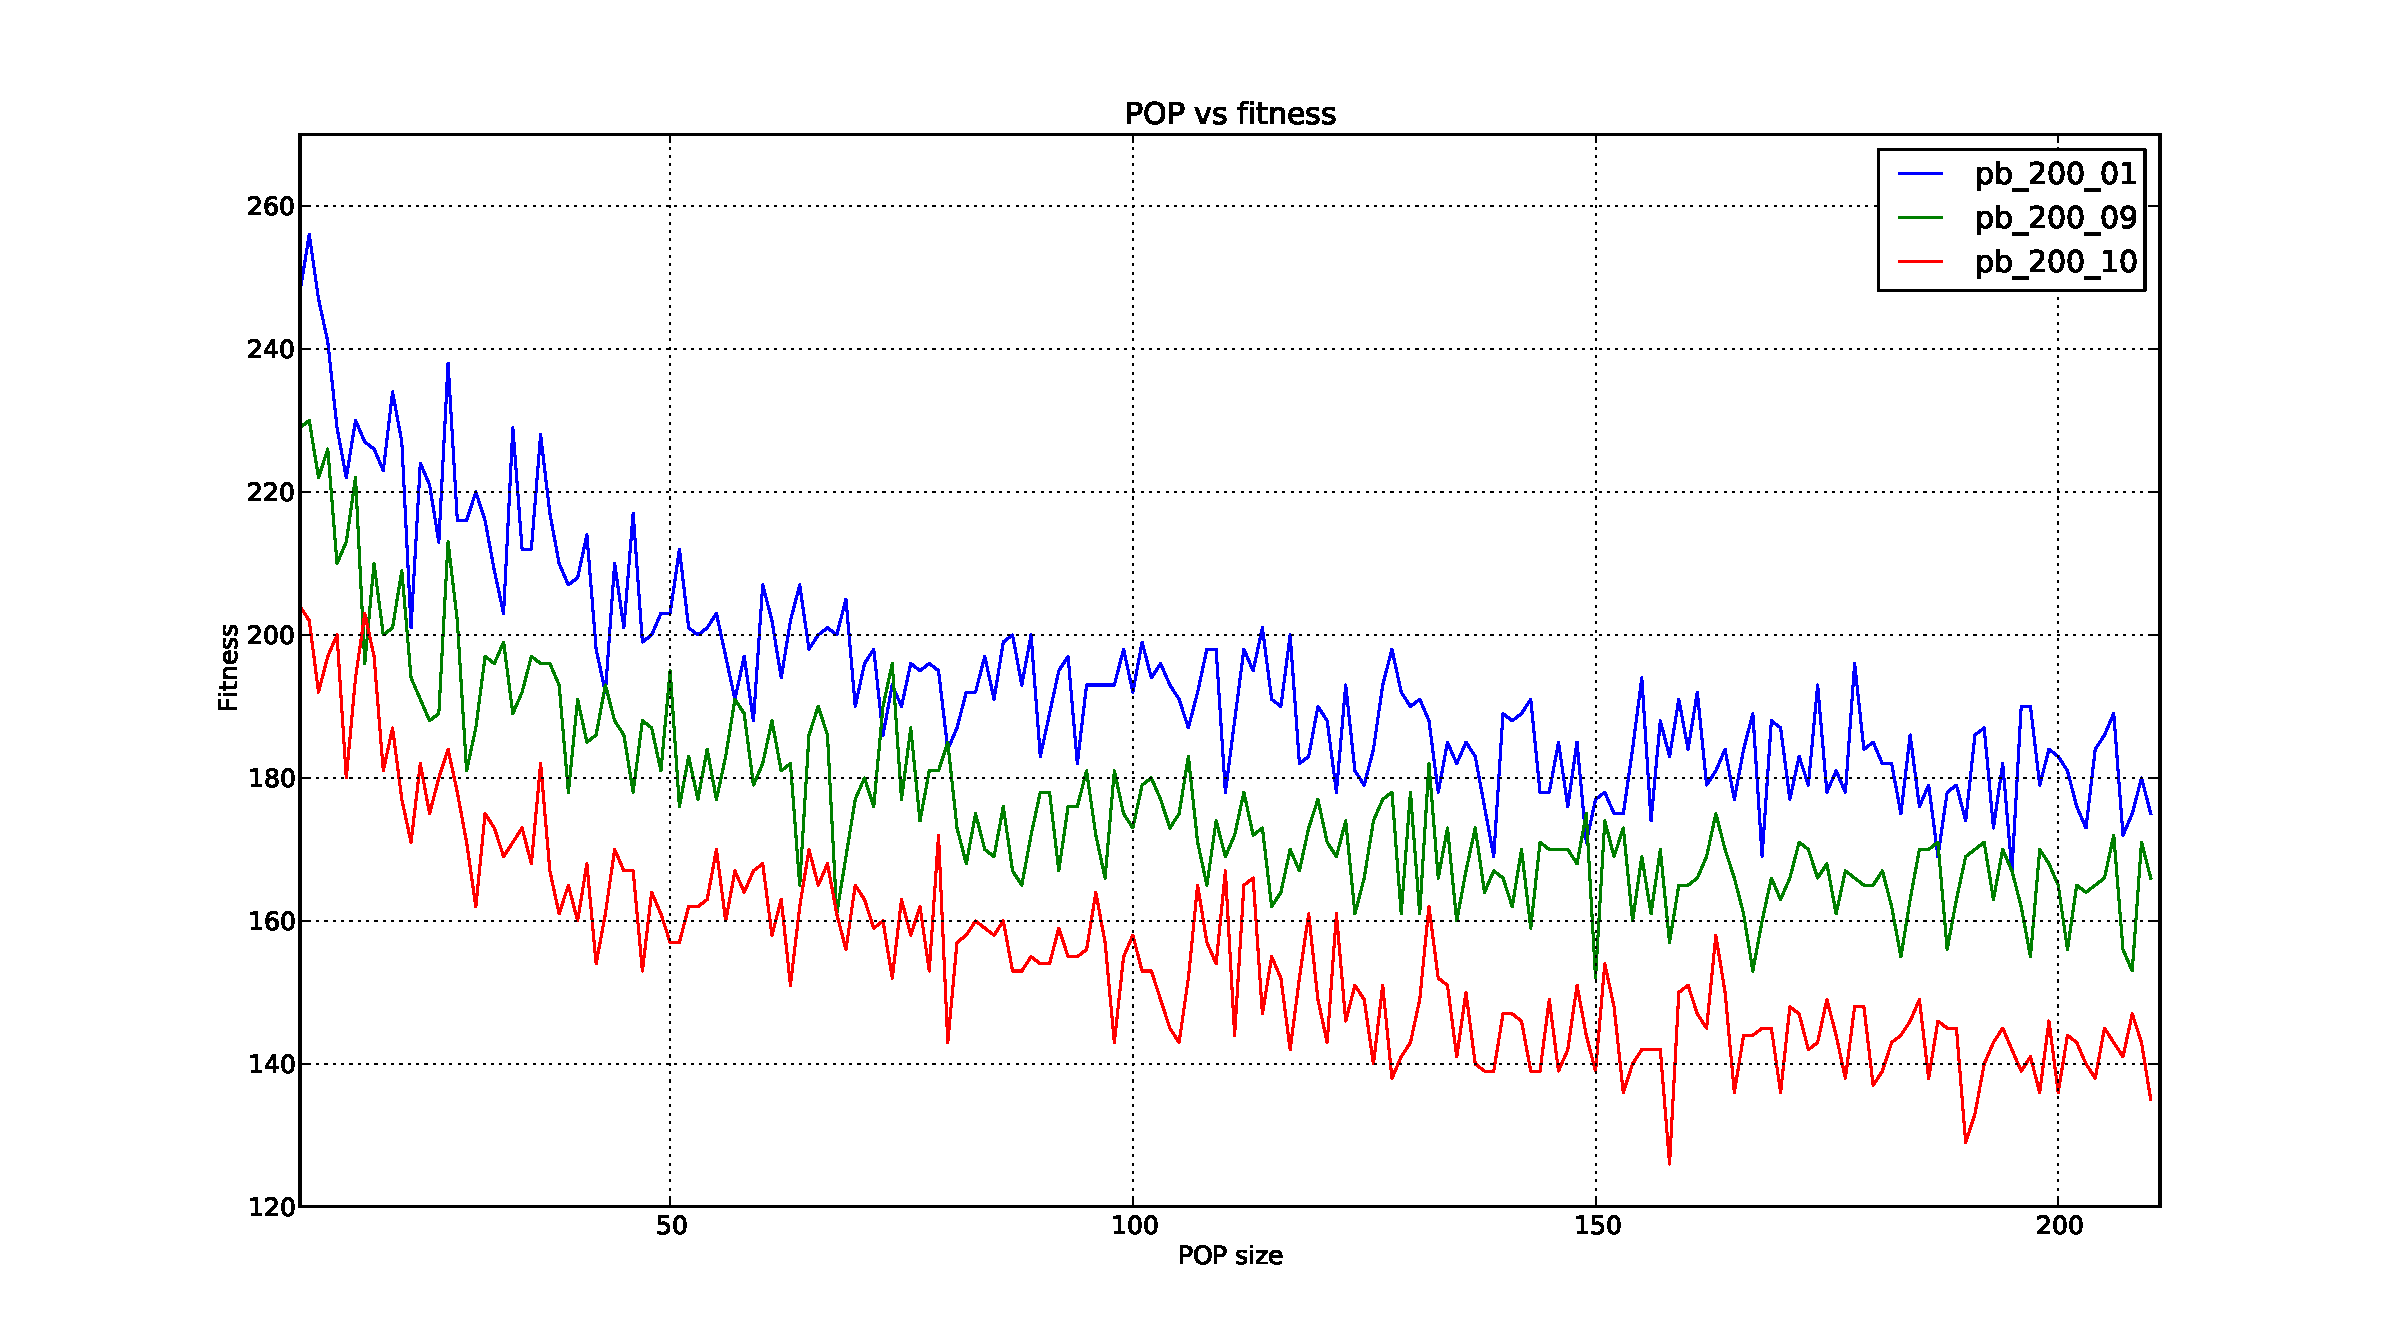
\includegraphics[width=0.95\textwidth]{img/1.pdf}
	\caption{Comparaci\'on de las tres instancias dado un cambio en la poblaci\'on}
	\label{fig:1}
\end{center}
\end{figure}

\textbf{Configuración escogida:}\\

La siguiente tabla, proporciona la información pertinente del mejor resultado obtenido,
de las $200$ iteraciones en las que consistió la presente prueba por cada instancia.

Gracias a la figura~\ref{fig:1}, podemos darnos cuenta del comportamiento que nuestro
algoritmo va teniendo a medida que vamos aumentando el tamaño de la población.

En un comienzo podemos ver el pésimo comportamiento que posee, pues como la cantidad de
la población es muy pequeña, los anticuerpos no van a poder variar mucho, ya que al
momento de clonar o introducir diversidad, no cumplen su objetivo principal, pues
como estos procedimiento van a depender netamente del tamaño de la población, no serán
del todo útiles.

Cabe señalar que en realidad el comportamiento que está tomando el algoritmo, es más
bien siempre trabajar con soluciones aleatorias, pues la hipermutación de los clones
está determianda por el índice de la población, por lo que el mayor individuo se mutará
muy poco, lo que llevará a obtener pocas mejoras en nuestros anticuerpos.


\begin{center}
\begin{tabular}{|l|c|c|c|c|}
	\hline
	\textbf{Instancia} & \textbf{POP} & \textbf{Mejor resultado} & \textbf{Tiempo [s] } & \textbf{Tiempo total [s] }\\\hline
	\texttt{pb\_200\_01.txt} & 195 & 167 & 15.110 & 1608.853 \\\hline 
	\texttt{pb\_200\_09.txt} & 150 & 152 & 11.243 & 1593.739 \\\hline
	\texttt{pb\_200\_10.txt} & 158 & 126 & 11.210 & 1662.580 \\\hline
\end{tabular}
\end{center}

Las iteraciones luego de un tamaño en la población sobre $100$ aproximadamente,
se comienzan a comportar de una forma más normalizada, y la pendiente de la curva que aproxima
al comportamiento del algoritmo, se vuelve cada vez menor, lo cual está representado en la tabla,
ya que claramente los mejores rendimientos por cada instancia están sobre una población de
tamaño $100$.

A pesar de lo distinta que son cada instancia, en nivel de complejidad, los tiempos que toman
cada una están bien parecidas, entre $11$ y $15$ segundos, por lo que no hay mayor diferencia.
\newpage
\subsubsection{Número de generaciones}

\textbf{Prueba}: \blue{prueba2}\\

\textbf{Parámetros involucrados:} Número de generaciones \texttt{(GENS)}.\\

\textbf{Objetivo:} Analizar el comportamiento de acuerdo a fitness y tiempo de ejecución del número de generaciones entre un rango de valores.\\

\textbf{Metodología:} Se probarán varios valores en el rango de valores del parámetro \blue{[10,2000]} (iterando de 30 en 30).\\

\textbf{Gráfico:}\\

\begin{figure}[h!]
\begin{center}
	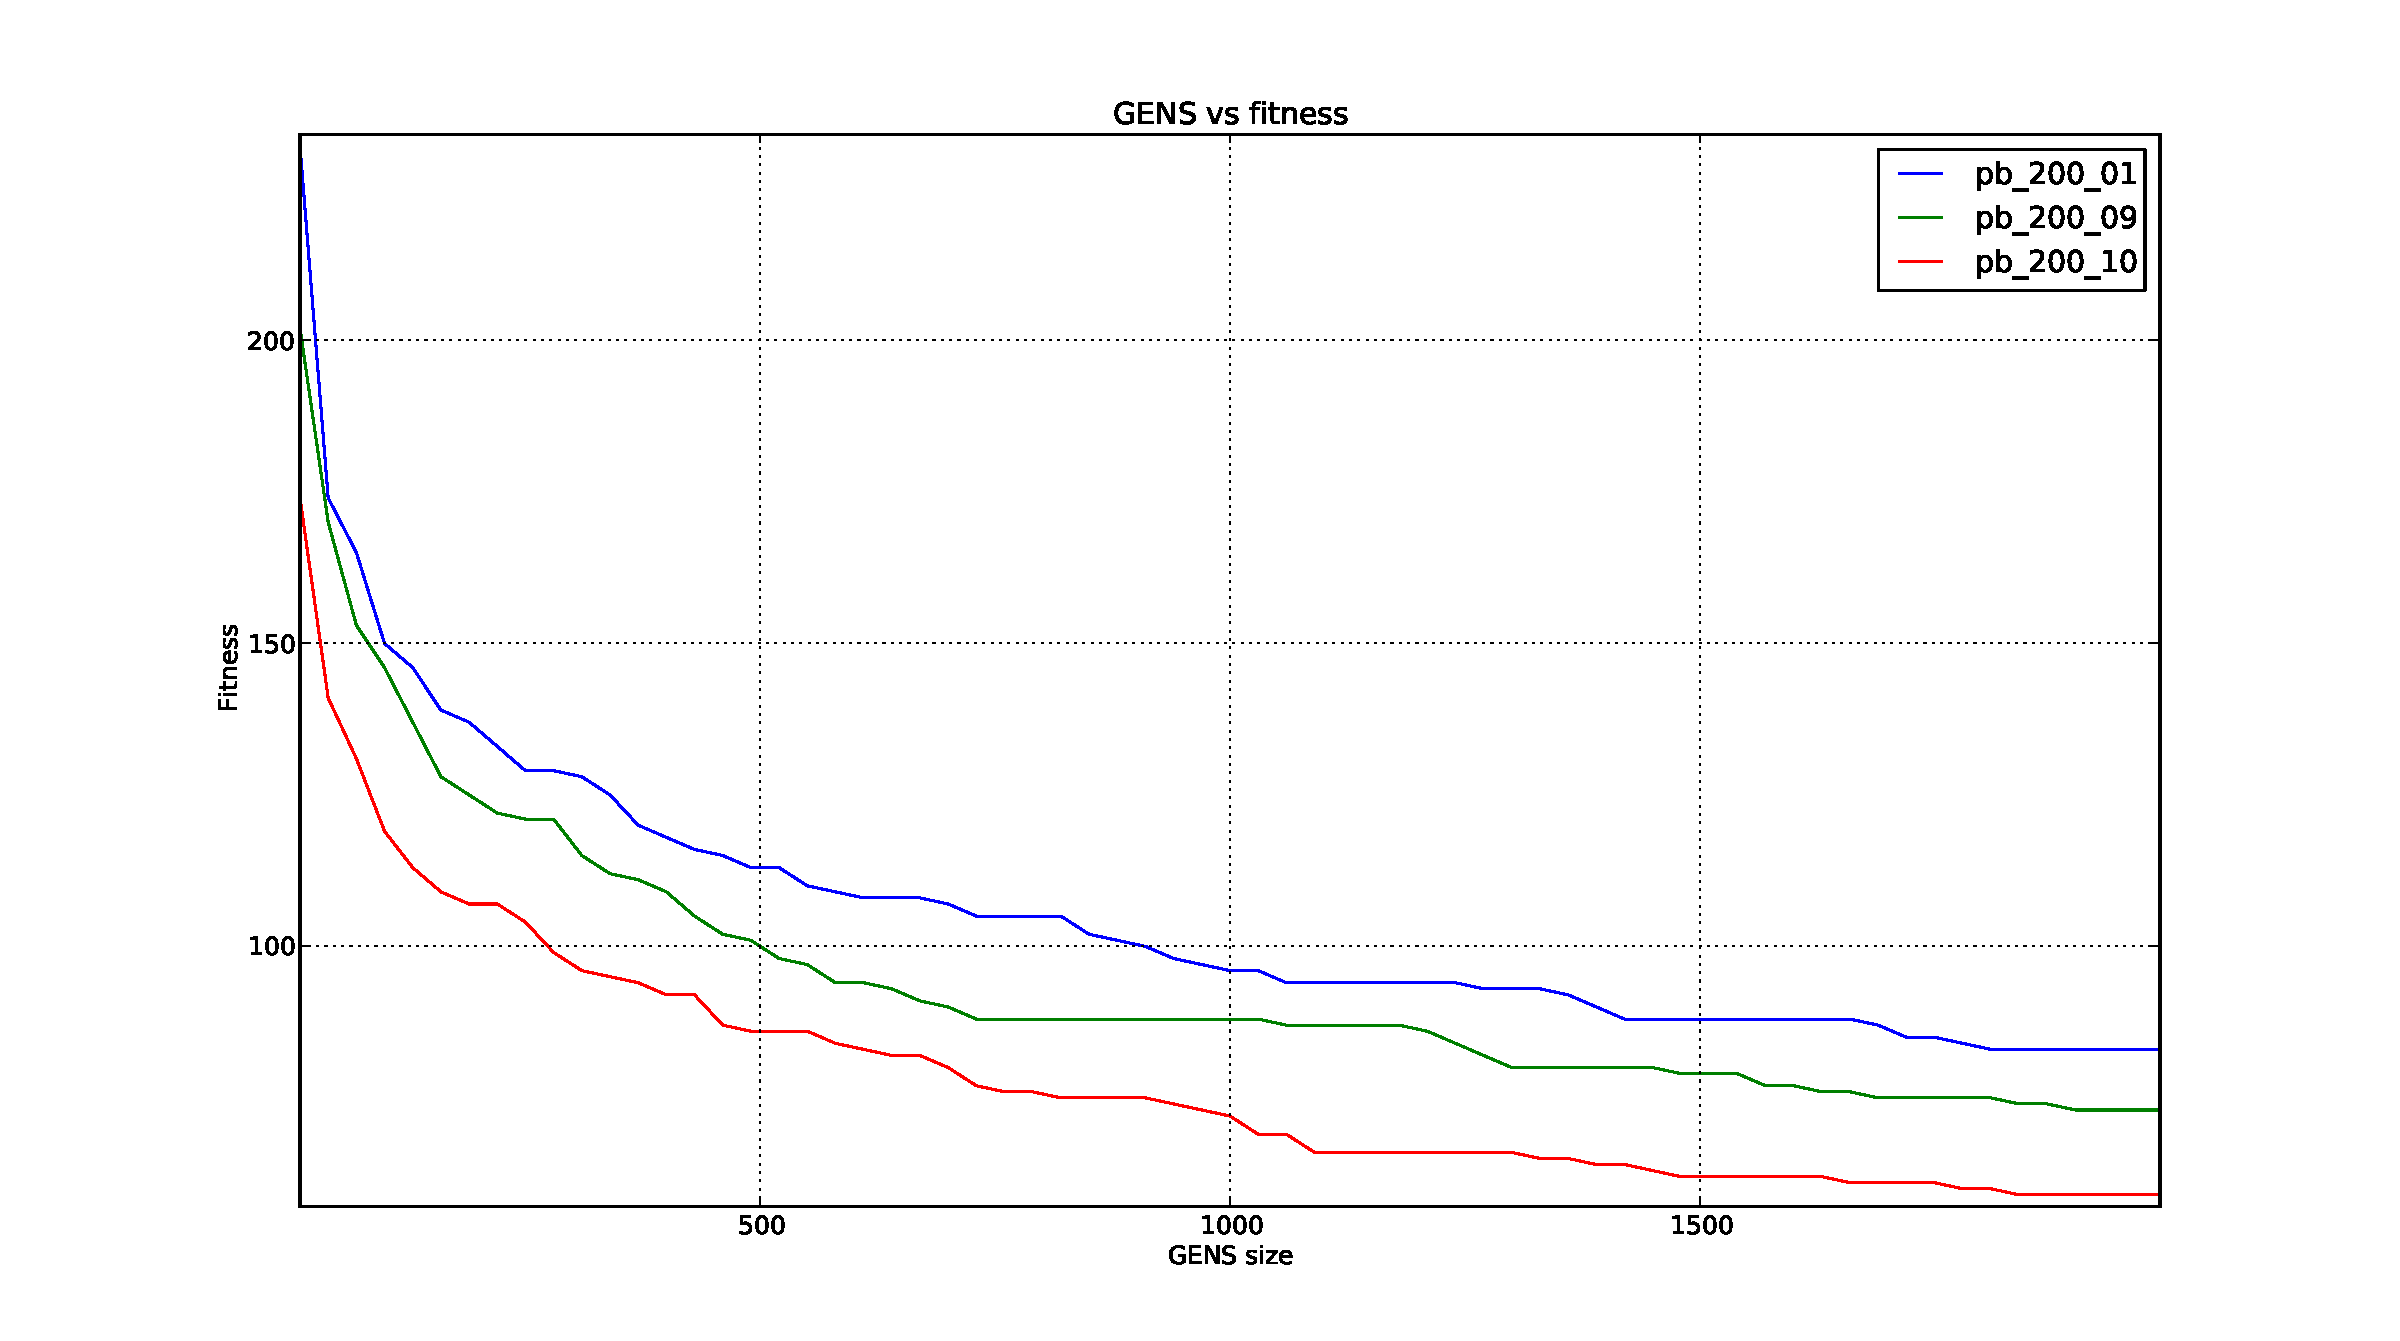
\includegraphics[width=0.95\textwidth]{img/2.pdf}
	\caption{Comparaci\'on de las tres instancias dado un cambio en el n\'umero de generaciones}
	\label{fig:2}
\end{center}
\end{figure}

\textbf{Configuración escogida:}\\

El gráfico~\ref{fig:2} nos muestra un comportamiento bastante adecuado a lo que debió pasar
en la realidad, si nos damos cuenta los primeros fitness son muy altos debido a que la cantidad
de iteraciones del algoritmo es muy poca, por lo que no se alcanza a desarrollar en su totalidad.

A medida que vamos aumentando la cantidad de generaciones nos vamos percatando que el fitness
comienza a disminuir casi como una exponencial inversa, lo cual tiene sentido pues mientras
más iteraciones tengamos, el algoritmo va a poder desarrollarse mucho más y llevar a cabo
un buen tratamiento de individuos.

Pero todo este procedimiento no consiste sólo en poder aumentar la cantidad de generaciones,
ya que si nos damos cuenta, pasado la mitad del gráfico el fitness sigue disminuyendo pero
en mucha menor cantidad que en un principio, lo uqe está perfecto para poder realizar
un control de parámetros en lo que són el número de generaciones, para saber
hasta que punto mi algoritmo se va a comportar de la misma forma.


\begin{center}
\begin{tabular}{|l|c|c|c|c|}
	\hline
	\textbf{Instancia} & \textbf{GENS} &\textbf{Mejor resultado} & \textbf{Tiempo [s] } & \textbf{Tiempo total [s]}\\\hline
	\texttt{pb\_200\_01.txt} & 1810 & 186 & 7.782 & 256.177 \\\hline
	\texttt{pb\_200\_09.txt} & 1960 & 166 & 8.460 & 262.906 \\\hline
	\texttt{pb\_200\_10.txt} & 1630 & 144 & 7.562 & 256.546 \\\hline
\end{tabular}
\end{center}

Luego de ver los valores, podemos darnos cuenta que el algoritmo se comporta bien con mas de 1500 generaciones,
por lo que podriamos considerar que desde ese punto el comportamiento es casi horizontal y que las mejoras
son muy pocas, con respecto al tiempo, este aumento bastante, lo que es obvio si pensamos que mientras
más iteraciones el problema se tomará más tiempo para hacer las mismas actividades muchas más veces.

Pero independiente del tiempo que aumento bastante, en términos generales el tiempo de ejecución sigue siendo
poco, sólo un par de segundos, lo que insita a poder probar el algoritmo con muchas más generaciones para
ver que tanto es el costo que debemos pagar en sentidos de tiempos, para obtener una buena solución.



\newpage
\subsubsection{Tasa de reemplazo}

\textbf{Prueba}: \blue{prueba3}\\

\textbf{Parámetros involucrados:} Tasa de reemplazo \texttt{(replaceRate)}.\\

\textbf{Objetivo:} Analizar el comportamiento de acuerdo a fitness y tiempo de ejecución de la tasa de reemplazo entre un rango de valores.\\

\textbf{Metodología:} Se probarán varios valores en el rango de valores del parámetro \blue{[0,1]}.
Para éste caso en particular, se ejecutó el algoritmo 10 veces por cada valor del parámetros y luego se seleccionó la mejor
para poder hacer el siguiente análisis.\\

\textbf{Gráfico:}\\

\begin{figure}[h!]
\begin{center}
	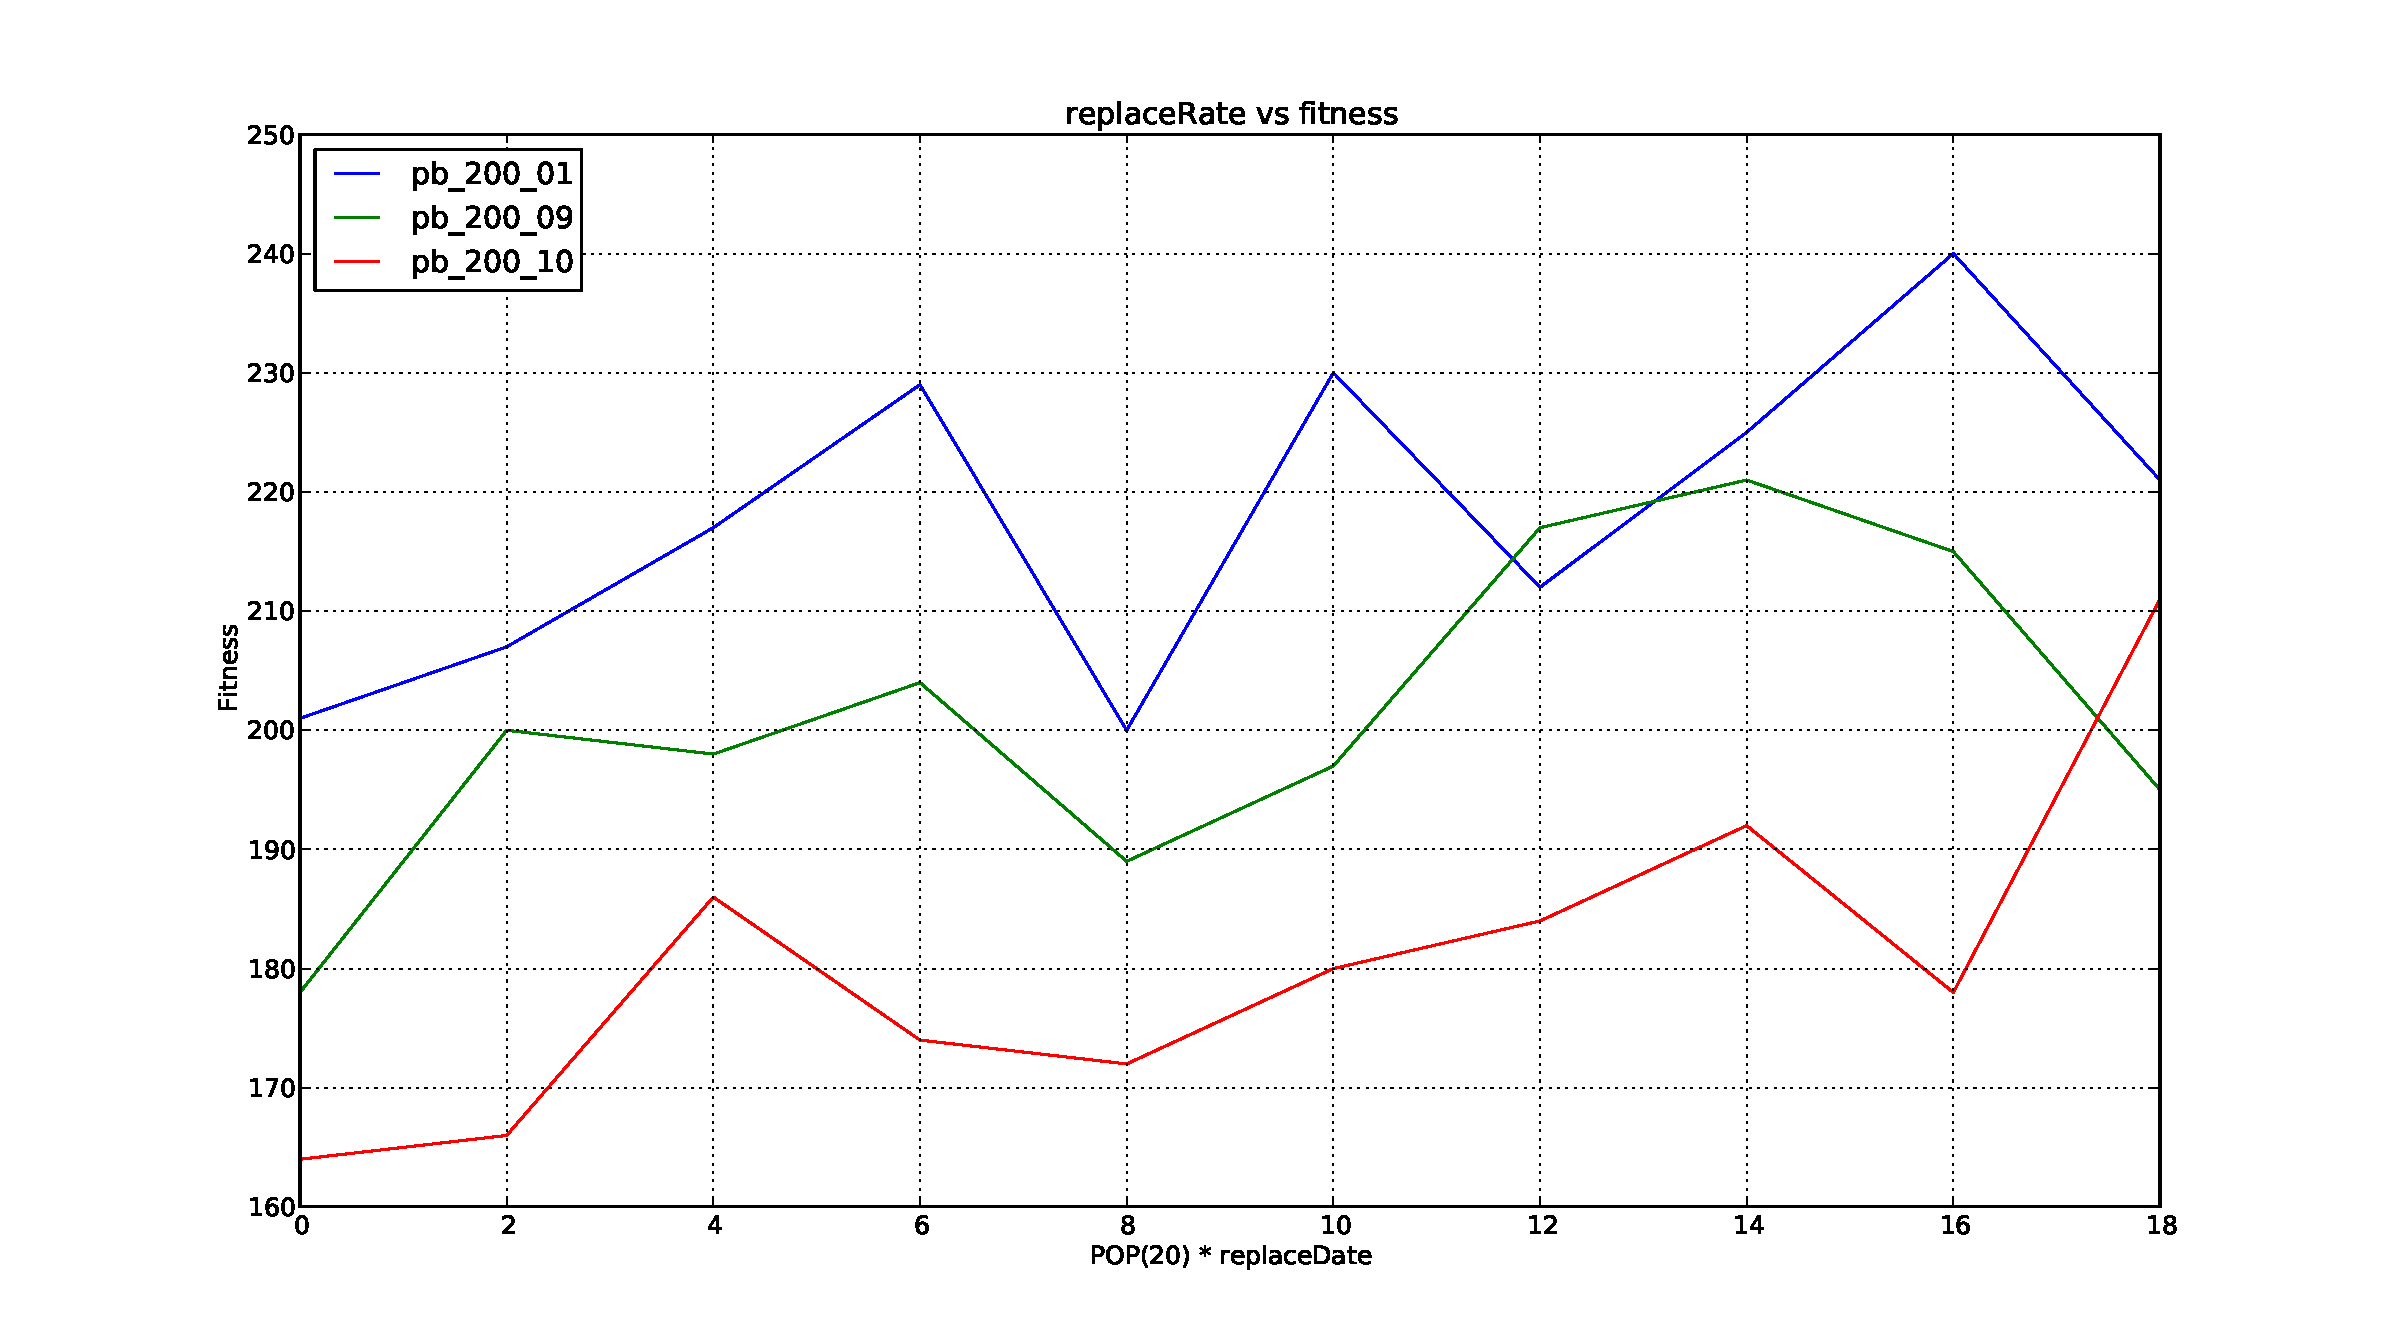
\includegraphics[width=0.95\textwidth]{img/3.pdf}
	\caption{Comparaci\'on de las tres instancias dado un cambio en la tasa de reemplazo}
	\label{fig:3}
\end{center}
\end{figure}

\textbf{Configuración escogida:}\\

La siguiente tabla, proporciona la información pertinente del mejor resultado obtenido,
de las $100$ iteraciones en las que consistió la presente prueba por cada instancia.

En éste caso, como se probaba la ``Tasa de reemplazo'' los valores posible son $0.1, 0.2, \ldots, 1.0$,
por lo que se realizó $10$ pruebas por cada valor.

Gracias a la figura~\ref{fig:3} nos podemos dar cuenta que los mejores valores se encuentran
para valores pequeños de la ``Tasa de reemplazo'' para las dos instancias finales, en cambio
para la primera instancia es un valor de $0.4$.

Podríamos ingenuamente decir, nuestro algoritmo no necesita ingresar diversidad y que por lo tanto
sólo nos dedicamos a \emph{explotar}, pero los resultados obtenidos se deben a que las iteraciones
que utilizamos como configuración básica son muy pocas, son sólo $200$, por lo que nuestro algoritmo
no alcanza a desarrollarse para poder tener la necesidad de salir de los ``óptimos locales'',
y así poder necesitar insertar diversidad, es por ésto que los valores de las dos últimas instancias,
es 0, pues el algoritmo no alcanza a necesitar diversidad.

\begin{center}
\begin{tabular}{|l|c|c|c|c|}
	\hline
	\textbf{Instancia} & \textbf{POP*replaceRate} & \textbf{Mejor resultado} & \textbf{Tiempo [s]} & \textbf{Tiempo total [s]}\\\hline
	\texttt{pb\_200\_01.txt} & 8 & 200 & 1.374 & 13.246 \\\hline
	\texttt{pb\_200\_09.txt} & 0 & 178 & 1.463 & 12.027 \\\hline
	\texttt{pb\_200\_10.txt} & 0 & 164 & 0.515 & 12.133   \\\hline
\end{tabular}
\end{center}

\newpage
\subsubsection{Factor de clonación y Tasa de clonación}

\textbf{Prueba}: \blue{prueba4} \\

\textbf{Parámetros involucrados}: Tasa de clonación y Factor de clonación. \\

\textbf{Objetivo}: Estudiar el efecto de la tasa y el factor de clonación en conjunto de acuerdo a fitness obtenido para la variación
de los dos parámetros en todo tu dominio.\\

\textbf{Metodología}: Se prueban varias combinaciones de valores para ver el efecto de los parámetros y poder observar su comportamiento.\\

\textbf{Configuración escogida:}\\

\begin{small}
\begin{center}
\begin{tabular}{|l|c|c|c|c|c|}
	\hline
	\textbf{Instancia} & \textbf{clonationRate} & \textbf{clonationFactor} &\textbf{Mejor resultado} & \textbf{Tiempo [s]} & \textbf{Tiempo total [s]}\\\hline
	\texttt{pb\_200\_01.txt} & 0.6 & 1   & 192 & 1.241 & 132.608 \\\hline
	\texttt{pb\_200\_09.txt} & 0.6 & 1   & 180 & 1.378 & 132.068 \\\hline
	\texttt{pb\_200\_10.txt} & 0.5 & 0.9 & 160 & 1.379 & 132.124 \\\hline
\end{tabular}
\end{center}
\end{small}
\normalsize
\textbf{Gráfico:}\\

\begin{figure}[h!]
\begin{center}
	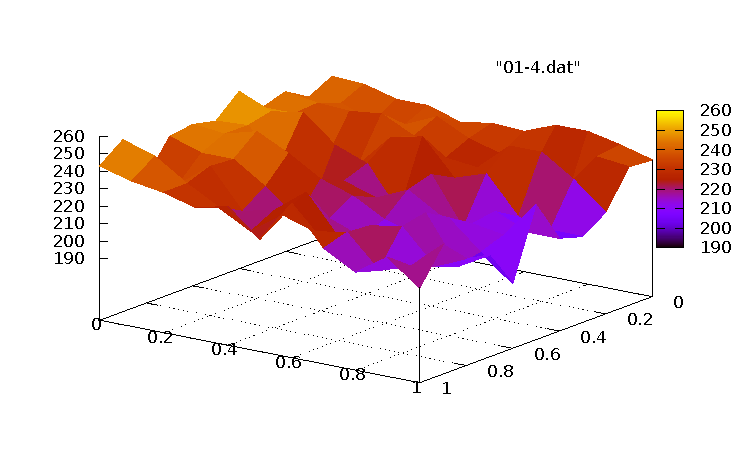
\includegraphics[width=0.95\textwidth]{img/01-4.pdf}
	\caption{Comparaci\'on de la instancia \texttt{pb\_200\_01.txt} variando \texttt{clonationRate} y \texttt{clonationFactor}}
	\label{fig:4-1}
\end{center}
\end{figure}

\begin{figure}[h!]
\begin{center}
	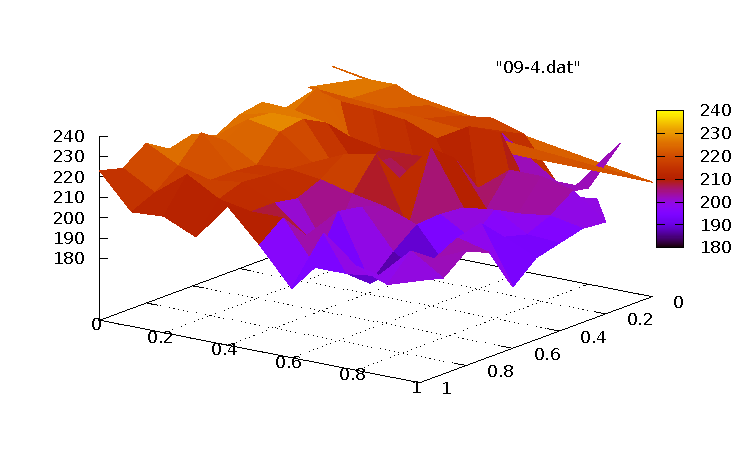
\includegraphics[width=0.95\textwidth]{img/09-4.pdf}
	\caption{Comparaci\'on de la instancia \texttt{pb\_200\_09.txt} variando \texttt{clonationRate} y \texttt{clonationFactor}}
	\label{fig:4-2}
\end{center}
\end{figure}

\begin{figure}[h!]
\begin{center}
	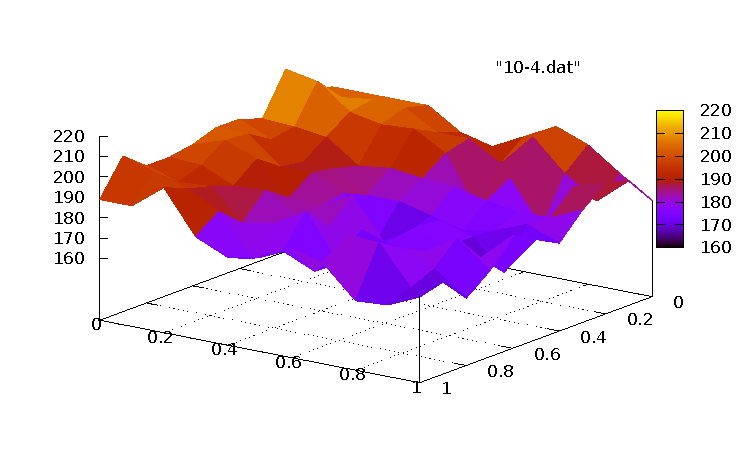
\includegraphics[width=0.95\textwidth]{img/10-4.pdf}
	\caption{Comparaci\'on de la instancia \texttt{pb\_200\_10.txt} variando \texttt{clonationRate} y \texttt{clonationFactor}}
	\label{fig:4-3}
\end{center}
\end{figure}

Si nos damos cuenta, cada una de los gráficos tiende a ser muy parecido,
pues siguen el patrón de para valores pequeños de los dos parámetros a sintonizar
el fitness es bastante alto, pero al momento de ir acercándose a valores que rodean a 1,
el fitness comienza a ser mucho mejor.

Es posible inferir que a medida que se aproximan los parámetros a 1, el algoritmo
comienza a a intensificar, razón por la cual comienza a entregar mejores generaciones y por ende
un mejor resultado.

Finalmente, sólo con la información del gráfico podemos darnos cuenta de que
para la ``Tasa de clonación'' y el ``Factor de clonación'' cercanos a 1,
el algoritmo se comporta de buena forma, por lo que a medida que vayamos aumentando
la cantidad de iteraciones podremos obtener mejores resultados, pero las mejoras
irán en disminución a medida que avancemos.

%
%
%elegir una configuración para cada instancia
%	-indicar el fitness
%	-identificar claramente las características del algoritmo.
%	-estimación del tiempo en realizarla.
\newpage

